\documentclass[UTF8]{ctexart}
\usepackage{graphicx}
\usepackage{float}
%opening
\title{系统分析与设计方法 \\ 作业 2}
\author{软件42 \\ 欧阳鹏程 \\ 2141601030}

\begin{document}

\maketitle

\begin{enumerate}
	\item
	请结合教材相关内容以及网络资料与课件,对网络中提供的一个需求管理系统进行分析,并尝试对整个系统中的实体以及属性进行建模,并对其特征进行定义。
\end{enumerate}
	\paragraph{答:} 以著名的需求管理软件Rational DOORS为例进行说明:
		\begin{figure}[H]
		\centering
		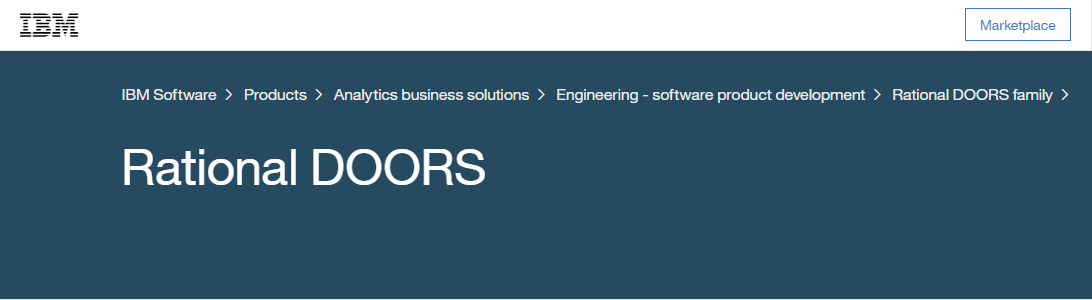
\includegraphics[width=0.9\textwidth]{1.png}
		\caption{Rational DOORS}
	\end{figure}
	\begin{enumerate}
		\item 什么是需求管理?
		需求管理是系统地收集与沟通所有项目目标及保证这些目标,且仅仅是这些目标被完全与正确地满足的相关活动。
		
		\item 为什么需求管理很关键?
		根据Standish 集团的工业报告“Extreme Chaos” (2001), 在2000 年只有28%的软件开发项目获得了成功。23%的软件开发项目是失败的,49%是“被质疑的”-就是说这些项目超过时限、超过预算或没有实现最初计划的功能。
		当Standish 集团问及项目成功的因素时,发现有44%的原因与需求直接相关。也就是说,有接近一半的原因来源于同一领域:需求管理。基于这样的数据,你无法不全心面对这一领域。
		
		\item Telelogic DOORS企业需求管理套件简介
		用于加快项目进程与提高项目质量的需求管理工具应当被紧密地结合到组织中。捕获、组织与确定关键信息的优先级不应该只由某一单一领域的工程师或分析师来完成。需求管理是团队的工作,只有这样才能保证统一的步调,使项目成功。
		Telelogic DOORS 企业需求管理套件(DOORS/ERS)是仅有的面向\textbf{管理者}、\textbf{开发者}与\textbf{最终用户}及整个生命周期的综合需求管理套件。
	
		\item DOORS/ERS 是灵活的解决方案
		具有以下功能:
		沟通
		协同
		无处不在的验证
		结果:
		缩短上市时间
		提高质量
		项目的成功能够被重复
		降低成本
		
		\item DOORS/ERS 可以使企业内部流畅地沟通需求
		通过DOORS/ERS,你能够无缝地把需求管理结合到拥有不同角色和责任的各类人员的工作中。无论他们对需求管理的经验水平如何:
		\subitem 需求分析工程师:他们是与写需求、进行需求工程或引出需求的相关人员,这些用户通常会用DOORS 写最初的需求或对需求进行分析。
		\subitem 系统/软件工程师:他们是那些在日常工作中直接使用需求的人;他们需要从DOORS 的数据中推导出与设计相关的需求。
		\subitem 测试工程师:负责确保结果的正确,测试工程师可以从DOORS中直接生成测试程序,或使用其它的工具管理测试,同时使用DOORS来帮助把测试与需求的关系建立起来。
		\subitem 销售与市场人员:负责前期把用户的需求反馈到DOORS/ERS 中,这些非技术用户可以轻松地使用DOORS 来完成他们的工作。
		\subitem 最终用户:往往在组织之外从事项目的工作,这些用户可以利用DOORS 对项目的进展进行跟踪、评判与建议-或使用DOORS提供原始的需求。
		\subitem 经理:根据他们对日常需求管理工作的参与程度而定,他们通常使用DOORS。
		\subitem 质量保证工程师:非常关心可跟踪性,这些用户可以利用DOORS 作为评审过程的关键部分。
		
		可以从DOORS/ERS 获益的用户:
		需求分析工程师,
		系统/软件工程师,
		测试工程师,
		最终用户,
		管理人员,	
		质量保证工程师。
	
		\item DOORS 的优势
		沟通
		通过直观的用户界面,用户可以方便地通过网络并行访问DOORS,并维护大量的管理对象(需求和关联信息)和连接。通过fish-eye 和MicrosoftWindows 资源管理器的图形方式管理视图,每一个用户都可以方便地定制他们想要看到的需求信息—使用图形和颜色。
	\end{enumerate}
	
	那么我们可以知道,在Rational DOORS中存在以下几类业务参与者:管理者、开发者与最终用户。
	对于这三类人,他们分别有以下属性:
	\begin{itemize}
		\item 管理者
		\begin{enumerate}
			\item Administrator Number
			\item Account Type
			\item Account Information
			\subitem .User Name
			\subitem .Password
			\subitem .Alias Name
			\subitem .Gender
			\subitem .Date of Birth
			\item Subordinates Charged
			\item Projects charged
			\subitem .Target Users
			\subitem .Documentations
		\end{enumerate}
	
		\item 开发者
		\begin{enumerate}
			\item Developer Number
			\item Account Type
			\item Account Information
			\subitem .User Name
			\subitem .Password
			\subitem .Alias Name
			\subitem .Gender
			\subitem .Date of Birth
			\item Role
			\item Parts charged
			\item Parts can See
			\subitem .Documentations
			\item My Administrators
		\end{enumerate}
	
		\item 最终用户
		\begin{enumerate}
			\item User Number
			\item Account Type
			\item Account Information
			\subitem .User Name
			\subitem .Password
			\subitem .Alias Name
			\subitem .Gender
			\subitem .Date of Birth
			\item Projects can See
			\subitem .Project Display effect
			\subitem .Project Documentation
			\subitem .Administrators
		\end{enumerate}
	\end{itemize}
	除了这三类实体之外,将这三类实体联系起来的还有一个实体:Project,其属性如下:
	\begin{enumerate}
		\item Project Number
		\item Administrators
		\item Parts
		\item Users
		\item Documentations
	\end{enumerate}
	当然,每一个Project会被分割成很多小的部分来由不同的人来完成,所以还有一个实体Part,其属性如下:
	\begin{enumerate}
		\item Part Number
		\item Project Belonged
		\item Documentations
		\item Developers
		\item Administrators
	\end{enumerate} 
	最后这些实体之间的实体关系图如下:
	\begin{figure}
		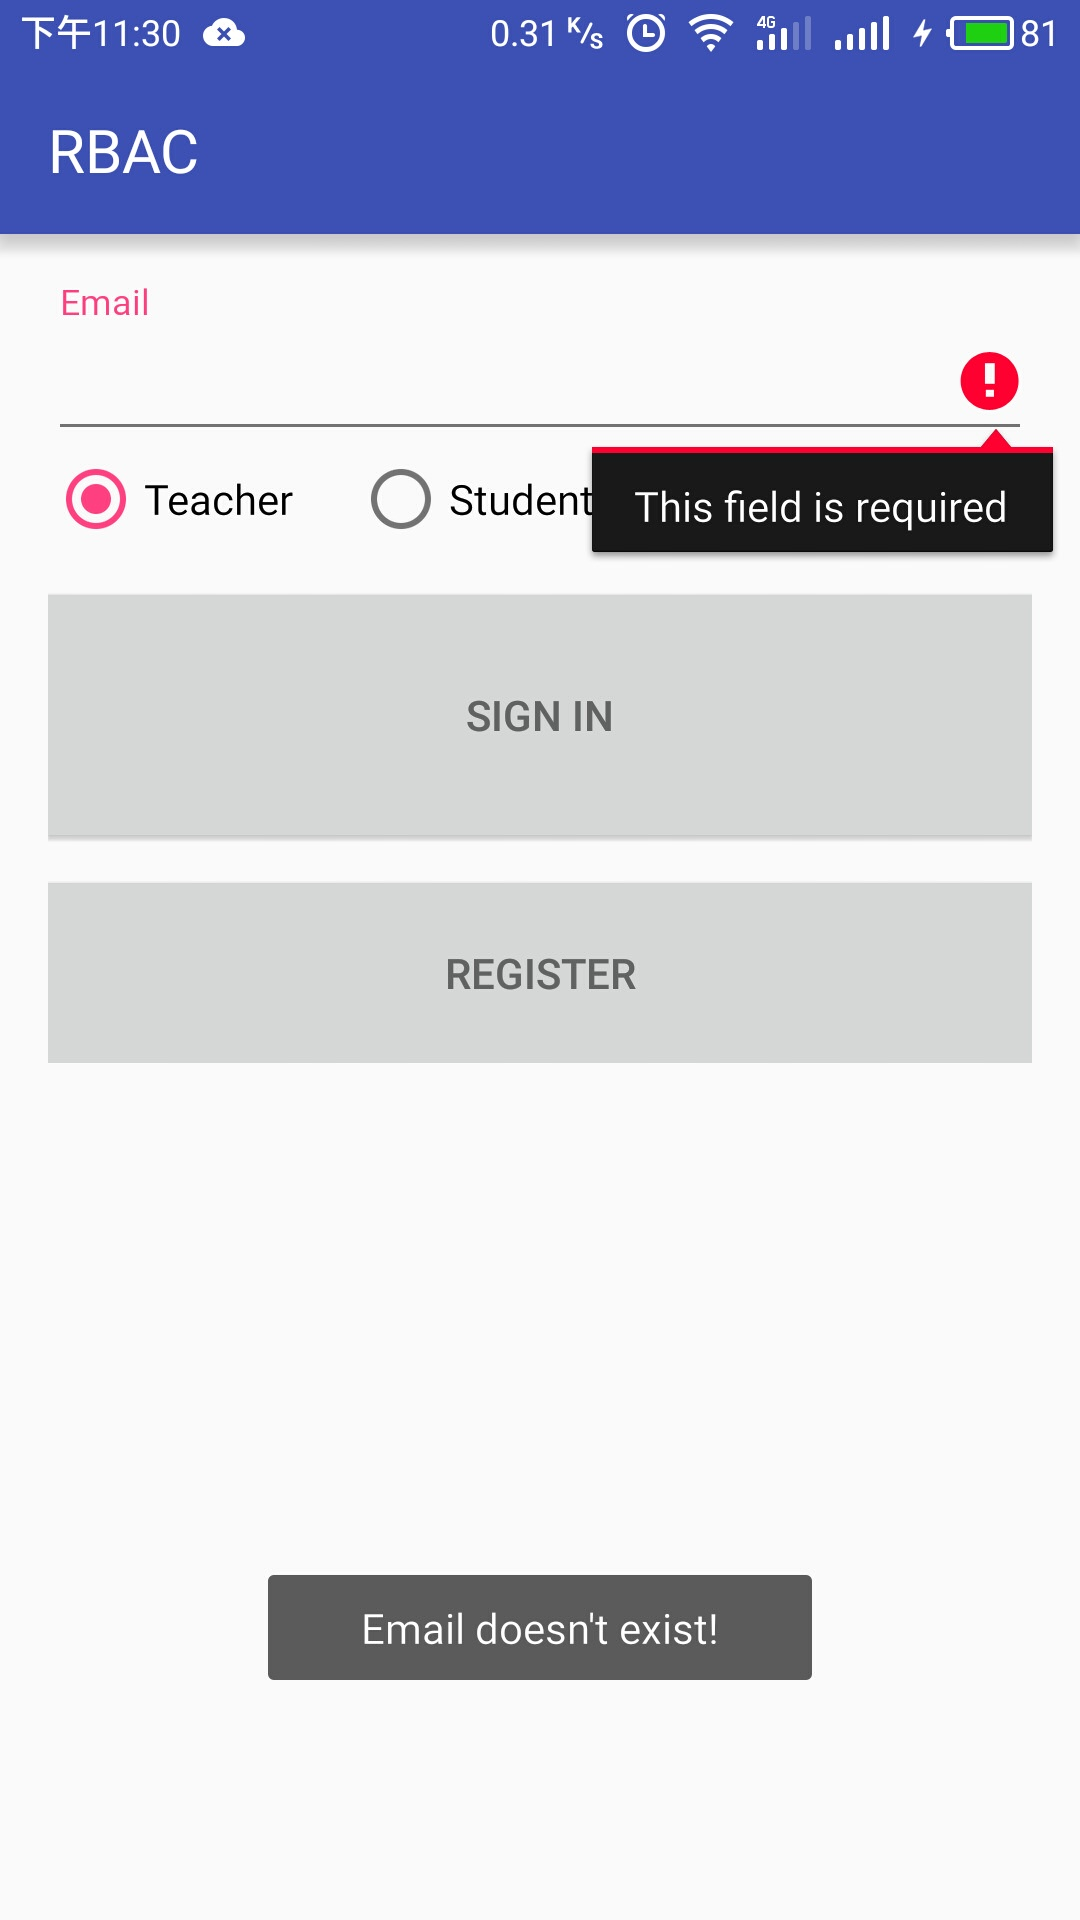
\includegraphics[width=\textwidth]{2.jpg}
		\caption{ER图}
	\end{figure}
\end{document}
